% !TEX encoding = UTF-8 Unicode
% !TEX TS-program = pdflatex

\documentclass{article}
	\usepackage{tikz}
	\usepackage{listings}
\begin{document}

	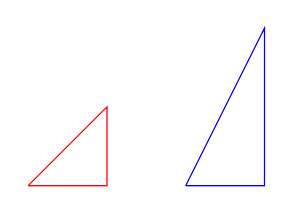
\begin{tikzpicture}
		\draw[red](0,0)--(1,0)--(1,1)--(0,0);
		\draw[blue](2,0)--(3,0)--(3,2)--(2,0);
	\end{tikzpicture}

\lstset{language=[latex]tex,tabsize=4}
\begin{lstlisting}
% !TEX encoding = UTF-8 Unicode
% !TEX TS-program = pdflatex
\documentclass{article}
	\usepackage{tikz}
\begin{document}
	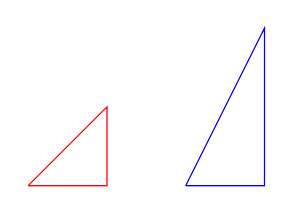
\begin{tikzpicture}
		\draw[red](0,0)--(1,0)--(1,1)--(0,0);
		\draw[blue](2,0)--(3,0)--(3,2)--(2,0);
	\end{tikzpicture}
\end{document}
\end{lstlisting}

\end{document}